\documentclass[10pt,journal,compsoc]{IEEEtran}

% === CRITICAL: ToUnicode mapping for correct text extraction ===
% cmap must be loaded BEFORE font packages to ensure proper character mapping
\usepackage{cmap}
% Enable glyph-to-unicode mapping (improves PDF text extraction fidelity)


\ifCLASSOPTIONcompsoc
  \usepackage[nocompress]{cite}
\else
  \usepackage{cite}
\fi
% Override Palatino with Times (required for IEEE TDSC)
\usepackage{mathptmx}
\usepackage{fix-cm}
\usepackage{amsmath,amssymb}
\usepackage{graphicx}
\usepackage{array}
\usepackage{booktabs}
\usepackage{url}
\usepackage{xurl}
\urlstyle{same}
\Urlmuskip=0mu
% Reset xurl's default lowercase breaks and use controlled break points only
\makeatletter
% Clear any lowercase letter break points that xurl may have added
% Note: Removed hyphen from UrlBreaks to prevent soft-hyphen artifacts (U+00AD) in extracted text
\def\UrlBreaks{\do\.\do\@\do\/\do\\\do\!\do_\do\|\do\;\do\>\do\]\do\)\do\,\do\?\do\'\do\+\do\=\do\#}
% Prefer breaking at path separators and colons
\def\UrlBigBreaks{\do\/\do\:}
% Do NOT add \UrlOrds or lowercase letters
\makeatother
\usepackage[T1]{fontenc}  % Better font encoding for text extraction
\usepackage[tracking=false,letterspace=0]{microtype}  % Disable letterspace to prevent char spreading
\microtypesetup{expansion=false}  % Disable font expansion for tt fonts
\usepackage[hidelinks]{hyperref}
% PDF Metadata for indexing and compliance
\hypersetup{
    pdftitle={},
    pdfauthor={},
    pdfkeywords={},
    pdfsubject={}
}
\usepackage{xr-hyper}
% Allow main paper to reference Supplementary Table/Figure numbers via \ref{}.
% Build supplementary.tex at least once so supplementary.aux exists.
\makeatletter
\IfFileExists{supplementary.aux}{\externaldocument{supplementary}}{}
\makeatother
\usepackage{xcolor}
\usepackage{fvextra}
\fvset{breaklines=true,breakanywhere=true,breakautoindent=false,breakindent=0pt,fontsize=\small}
\newcommand{\VerbBar}{|}
\newcommand{\VERB}{\Verb[commandchars=\\\{\}]}
\DefineVerbatimEnvironment{Highlighting}{Verbatim}{commandchars=\\\{\},breaklines=true,breakanywhere=true,breakautoindent=false,breakindent=0pt,fontsize=\small}
\newenvironment{Shaded}{}{}
\newcommand{\AlertTok}[1]{\textcolor[rgb]{1.00,0.00,0.00}{\textbf{#1}}}
\newcommand{\AnnotationTok}[1]{\textcolor[rgb]{0.38,0.63,0.69}{\textbf{\textit{#1}}}}
\newcommand{\AttributeTok}[1]{\textcolor[rgb]{0.49,0.56,0.16}{#1}}
\newcommand{\BaseNTok}[1]{\textcolor[rgb]{0.25,0.63,0.44}{#1}}
\newcommand{\BuiltInTok}[1]{\textcolor[rgb]{0.00,0.50,0.00}{\textbf{#1}}}
\newcommand{\CharTok}[1]{\textcolor[rgb]{0.25,0.44,0.63}{#1}}
\newcommand{\CommentTok}[1]{\textcolor[rgb]{0.38,0.63,0.69}{\textit{#1}}}
\newcommand{\CommentVarTok}[1]{\textcolor[rgb]{0.38,0.63,0.69}{\textbf{\textit{#1}}}}
\newcommand{\ConstantTok}[1]{\textcolor[rgb]{0.53,0.00,0.00}{#1}}
\newcommand{\ControlFlowTok}[1]{\textcolor[rgb]{0.00,0.44,0.13}{\textbf{#1}}}
\newcommand{\DataTypeTok}[1]{\textcolor[rgb]{0.56,0.13,0.00}{#1}}
\newcommand{\DecValTok}[1]{\textcolor[rgb]{0.25,0.63,0.44}{#1}}
\newcommand{\DocumentationTok}[1]{\textcolor[rgb]{0.73,0.13,0.13}{\textit{#1}}}
\newcommand{\ErrorTok}[1]{\textcolor[rgb]{1.00,0.00,0.00}{\textbf{#1}}}
\newcommand{\ExtensionTok}[1]{#1}
\newcommand{\FloatTok}[1]{\textcolor[rgb]{0.25,0.63,0.44}{#1}}
\newcommand{\FunctionTok}[1]{\textcolor[rgb]{0.02,0.16,0.49}{#1}}
\newcommand{\ImportTok}[1]{\textcolor[rgb]{0.00,0.50,0.00}{\textbf{#1}}}
\newcommand{\InformationTok}[1]{\textcolor[rgb]{0.38,0.63,0.69}{\textbf{\textit{#1}}}}
\newcommand{\KeywordTok}[1]{\textcolor[rgb]{0.00,0.44,0.13}{\textbf{#1}}}
\newcommand{\NormalTok}[1]{#1}
\newcommand{\OperatorTok}[1]{\textcolor[rgb]{0.40,0.40,0.40}{#1}}
\newcommand{\OtherTok}[1]{\textcolor[rgb]{0.00,0.44,0.13}{#1}}
\newcommand{\PreprocessorTok}[1]{\textcolor[rgb]{0.74,0.48,0.00}{#1}}
\newcommand{\RegionMarkerTok}[1]{#1}
\newcommand{\SpecialCharTok}[1]{\textcolor[rgb]{0.25,0.44,0.63}{#1}}
\newcommand{\SpecialStringTok}[1]{\textcolor[rgb]{0.73,0.40,0.53}{#1}}
\newcommand{\StringTok}[1]{\textcolor[rgb]{0.25,0.44,0.63}{#1}}
\newcommand{\VariableTok}[1]{\textcolor[rgb]{0.10,0.09,0.49}{#1}}
\newcommand{\VerbatimStringTok}[1]{\textcolor[rgb]{0.25,0.44,0.63}{#1}}
\newcommand{\WarningTok}[1]{\textcolor[rgb]{0.38,0.63,0.69}{\textbf{\textit{#1}}}}
\newcommand{\pandocbounded}[1]{#1}
\usepackage{calc}
\newcommand{\real}[1]{#1}
\providecommand{\tightlist}{%
  \setlength{\itemsep}{0pt}\setlength{\parskip}{0pt}}
\usepackage{tikz}
\usetikzlibrary{arrows.meta,positioning,shapes.geometric,calc,fit}

% Submission format: suppress running headers and page numbers.
% IEEEtran (journal) defaults to headers with page numbers; some venues prefer a clean manuscript PDF.
\makeatletter
\def\ps@headings{%
  \let\@oddhead\@empty
  \let\@evenhead\@empty
  \let\@oddfoot\@empty
  \let\@evenfoot\@empty
}
\def\ps@IEEEtitlepagestyle{%
  \let\@oddhead\@empty
  \let\@evenhead\@empty
  \let\@oddfoot\@empty
  \let\@evenfoot\@empty
}
\makeatother
\pagestyle{headings}

% Normalize list indentation for two-column IEEE layout.
\setlength{\leftmargini}{1.3em}
\setlength{\leftmarginii}{1.1em}
\setlength{\labelsep}{0.4em}
\setlength{\parindent}{1em}
\raggedbottom

% Prevent hyphenation of technical terms (no hyphens = no break points)
\hyphenation{keyShares supportedSuites enforceable downgrade guaranteeing implementation handshake CryptoProvider TranscriptIntegrityPropertyTests device auditable acceptance mature post-quantum pre-authentication authentication crypto-agile Legacy reference property oriented including demonstrates available consolidated benchmarks coverage CryptoKit}

% Paragraph breaking tuning: avoid extreme inter-word spacing in narrow columns.
\tolerance=1000
\emergencystretch=1em

% Non-breaking inline code (prevents line breaks inside technical identifiers)
\newcommand{\nbcode}[1]{\mbox{\texttt{#1}}}

\newcommand{\artifacturl}{https://github.com/billlza/Skybridge-Compass}
\newcommand{\artifacturlshort}{https://github.com/billlza/Skybridge-Compass}
\newcommand{\artifacttag}{artifact-v1}
\newcommand{\artifactsha}{8a68fa6e0fe7}
\newcommand{\artifactshafull}{8a68fa6e0fe78147d2b18d3287681f5d07c74afd}
\newcommand{\artifactzipurl}{\artifacturl/archive/refs/tags/\artifacttag.zip}
\newcommand{\artifactzipsha}{354443f7cda3e25a51480a683da1712a8ea9588a2bc510f4f716bd553d6d72ac}
\newcommand{\artifacttarurl}{\artifacturl/archive/refs/tags/\artifacttag.tar.gz}
\newcommand{\artifacttarsha}{90228458587f095e9cd403d3d449f885a2b8b002057a76e6f60c291e45071388}

\newcommand{\artifactcsv}[1]{\texttt{#1_2026-01-16.csv}}
\newcommand{\artifactpath}[1]{\texttt{Artifacts/#1_2026-01-16.csv}}
\newcommand{\implref}[2]{Implementation reference: \href{\artifacturl}{\artifacturlshort} (tag=\texttt{\artifacttag}, commit=\texttt{\artifactsha}), file: \texttt{#1}, lines: #2.}


\title{SkyBridge Compass: A Crypto-Agile Peer-to-Peer Remote Desktop and File Transfer System with Auditable Downgrade Policy and Post-Quantum Readiness}
\author{Zi'ang Li\IEEEcompsocitemizethanks{\IEEEcompsocthanksitem Independent Researcher, Tianjin, China. E-mail: 2403871950@qq.com.}}

\begin{document}


\begin{abstract}
Peer-to-peer remote desktop and file transfer
systems increasingly operate across heterogeneous devices, untrusted
networks, and long lifecycles in which cryptographic assumptions may
expire faster than products. Yet ``post-quantum readiness'' is often
treated as a one-off algorithm swap rather than a migration problem with
downgrade resistance, auditability, and reproducibility requirements.
This paper presents SkyBridge Compass, a crypto-agile P2P system that
explicitly separates (i) negotiated cryptographic suites, (ii)
provider backends, and (iii) a policy layer that governs when (and
whether) classic fallback is permissible. We use an actor-isolated
handshake state machine with deterministic outcomes and structured
security-event emission, enabling \mbox{end-to-end} audit trails for
downgrade, identity mismatch, and signature verification failures. We
evaluate three configurations on macOS 26.x as a deployment instance:
classic (X25519 + Ed25519), PQC via liboqs (ML-KEM-768 + ML-DSA-65), and
PQC via native CryptoKit (ML-KEM-768 + ML-DSA-65). We do not claim
perfect forward secrecy for the KEM-based PQC suites in v1; post-quantum
confidentiality holds only while long-term KEM private keys remain
uncompromised. \mbox{End-to-end}
handshake completion latency (including event emission overhead) is
1.62 ms (p95 1.81 ms) for classic, 2.29 ms (p95 3.01 ms) for liboqs PQC,
and 5.76 ms (p95 6.71 ms) for CryptoKit PQC over N=1000 iterations.
The handshake wire size (MessageA + MessageB + 2×Finished) grows
from 827 B (classic) to 12,163 B (PQC); X-Wing hybrid KEM measures
12,195 B. Beyond
performance, we validate downgrade policies, failure semantics, and
audit-signal fidelity under fault injection, and we release scripts and
artifacts that reproduce all primary figures and tables.
\end{abstract}

\begin{IEEEkeywords}
post-quantum cryptography, crypto agility, downgrade resistance, secure handshake, peer-to-peer systems, remote desktop, auditability, reproducibility, platform deployment.
\end{IEEEkeywords}

\maketitle


\section{Introduction}\label{sec:introduction}

\noindent Peer-to-peer (P2P) remote desktop and file transfer systems must
establish secure sessions under adversarial network conditions, device
churn, and multi-year lifecycles. These systems face a practical
tension: users demand ``it just works'' pairing across heterogeneous
stacks, while defenders require that cryptographic negotiation remains
robust against downgrade and \mbox{implementation-level} failure modes.
Post-quantum cryptography (PQC) increases this tension. Larger messages,
higher computational cost, and uneven platform support make fallback
tempting---yet fallback is exactly where silent downgrade and
unverifiable behavior tend to hide.

Existing secure-channel designs and frameworks provide mature
cryptographic building blocks, but they do not, by default, solve the
migration problem an implementer actually faces: (i) selecting among
classic/PQC/hybrid suites across platform strata, (ii) ensuring that
policy (e.g., ``require PQC'') is enforced at the entry points where
callers cannot accidentally violate it, (iii) targeting deterministic
failure semantics under timeouts, reorder/duplication, and malformed
inputs, and (iv) emitting security-relevant telemetry that can be
audited without turning the system into a logging minefield. In
practice, many systems either hard-code a single suite, or allow
``compatibility'' to creep into negotiation in ways that are hard to
reason about and harder to verify.

This paper addresses these gaps with SkyBridge Compass, a crypto-agile
P2P system designed for explicit PQC migration and auditability, with
Apple platforms as a deployment instance. The core idea is to treat
crypto agility as a layered
contract: negotiated suites define the protocol surface; provider
backends implement suites using platform-native or portable
cryptography; and a policy layer governs fallback and produces
structured evidence when (and only when) downgrade occurs. We complement
this design with an actor-isolated handshake driver that enforces
one-shot completion, timeouts, and sensitive-material zeroization,
yielding deterministic outcomes under the modeled transport faults.

\textbf{Security Guarantees (Checklist).}
To reduce ambiguity in reviewer-facing claims, we state the v1 guarantees
as a checklist of \emph{verifiable} properties under the threat model in
Section~5:
{\small
\begin{itemize}\tightlist
\item \textbf{Negotiation integrity:} the Responder selects only a suite
  offered by the Initiator and with a matching key share; unknown suite
  IDs are rejected if they appear in \nbcode{keyShares[]} or as
  \texttt{selectedSuite}. \textit{Evidence:} Fig.~1;
  Table~3;
  \texttt{HandshakeDriverTests}.
\item \textbf{Transcript binding:} \texttt{sigB} commits to MessageA and
  the chosen suite (and policy), so any tampering of
  \nbcode{supportedSuites[]}, \nbcode{keyShares[]}, or \texttt{policy}
  fails verification. \textit{Evidence:} Table~3;
  \texttt{TranscriptIntegrityPropertyTests};
  \texttt{ProtocolSignatureRegressionTests}.
\item \textbf{Downgrade resistance (policy-defined):} \texttt{strictPQC}
  forbids all fallback; the default policy permits fallback only for a
  local-only whitelist of capability/provider failures (timeouts and
  unauthenticated network failures cannot trigger fallback).
  \textit{Evidence:} Fig.~4; Fig.~5;
  \texttt{PolicyDowngradeBenchTests};
  Table~6.
\item \textbf{Explicit key confirmation:} two Finished frames provide
  mutual confirmation, preventing half-open sessions (Fig.~1).
  \textit{Evidence:} Table~5;
  \texttt{HandshakeFaultInjectionBenchTests}.
\item \textbf{Auditability of migration decisions:} every fallback emits
  a structured \texttt{cryptoDowngrade} event with a minimal evidence
  tuple (Section~5), enabling post-hoc verification
  and detection (e.g., Fig.~7). \textit{Evidence:}
  Fig.~7; Table~3.
\item \textbf{Non-claims (scope control):} v1 does \emph{not} claim PQC
  PFS for KEM-to-static-recipient suites, nor tamper-evident audit logs;
  see Section~8.
\end{itemize}
}

\subsection{Contributions}\label{a.-contributions}

Contributions:

\begin{enumerate}
\item
  We turn PQC migration from a narrative into an enforceable contract by
  making downgrade and \mbox{legacy-compatibility} decisions explicit,
  testable, and auditable rather than implicit ``best-effort'' fallback.
  \textit{Evidence:} Fig.~5; Table~3;
  \\
  \texttt{PolicyDowngradeBenchTests},\\
  \texttt{LegacyFallbackPreconditionTests}.
\item
  We design a crypto-agile P2P handshake that cleanly separates suite
  negotiation, transcript binding, and protocol-signature keys,
  preventing ``suite says PQC but keys stay classical'' class of
  integration bugs. \textit{Evidence:} Fig.~1; Table~3;
  \\
  \texttt{ProtocolSignatureRegressionTests},\\
  \texttt{TranscriptIntegrityPropertyTests}.
\item
  We provide migration safety with measurable coverage by enumerating
  legacy/PQC strata and validating acceptance/rejection boundaries under
  fault injection instead of relying on informal compatibility claims.
  \textit{Evidence:} Table~6; Table~5;
  \\
  \texttt{HandshakeFaultInjectionBenchTests}.
\item
  We harden correctness under concurrency by an actor-isolated state
  machine with idempotent transitions and bounded retries, eliminating
  double-resume and state desynchronization failure modes. \textit{Evidence:} Fig.~3;
  \\
  Table~3; \texttt{HandshakeDriverTests}.
\item
  We make evaluation reproducible by shipping a benchmark harness that
  reports distributional statistics (p50/p95/p99) over large-N runs and
  links each metric back to a concrete failure taxonomy.
  \textit{Evidence:} Fig.~4; Table~8;
  \\
  \texttt{HandshakeBenchmarkTests},\\
  \texttt{MessageSizeSnapshotTests}.
\end{enumerate}

\subsection{Paper Organization}\label{b.-paper-organization}

Section~2 reviews related work on P2P pairing,
negotiation, and PQC migration. Section~3
details system architecture and protocol design.
Section~4 presents the handshake state
machine. Section~5 presents the security model
and guarantees. Section~6 describes
implementation highlights and platform instantiation. Section~7
outlines evaluation methodology and metrics. Section~8
discusses limitations and future work, and Section~9
concludes. Supplementary Materials provide full wire-format definitions,
implementation details, and extended tables.



\section{Related Work}\label{sec:related-work}

We use the following terms throughout: \emph{crypto agility} (ability to
migrate primitives without redesign), \emph{downgrade resistance}
(prevent or detect forced fallback), \emph{suite negotiation} (explicit,
authenticated selection of handshake KEM/SIG/AEAD/KDF), \emph{PQC readiness}
(ability to deploy PQC alongside classic suites), and \emph{auditability}
(deterministic, minimal event traces for security decisions). Our threat
model assumes an active network attacker attempting to induce fallback
or obscure failures; therefore we focus on mechanisms that make
negotiation and failures explicit and auditable.

\subsection{Peer-to-Peer Device
Pairing}\label{a.-peer-to-peer-device-pairing}

Pairing protocols such as Bluetooth SSP [2], Continuity [3],
and PAKEs like SPAKE2+ [4] establish initial trust but stop short
of post-pairing migration, downgrade policy, or auditability. SkyBridge
Compass begins \emph{after} pairing and treats pinned identity keys as
inputs rather than outcomes.

\subsection{Cryptographic Agility and
Negotiation}\label{b.-cryptographic-agility-and-negotiation}

TLS 1.3 and QUIC bind negotiated parameters into transcripts and
transport parameters to prevent silent downgrade [6], [18],
but they do not define an auditable, system-level fallback policy across
heterogeneous providers. We operationalize migration guidance
[7, 38] with explicit policy gates and event emission that make
downgrade decisions observable and testable.

\subsection{Handshake Frameworks and Noise-Style
Patterns}\label{c.-handshake-frameworks-and-noise-style-patterns}

Noise provides a compact framework for describing authenticated key
exchange patterns with explicit transcript binding and identity key
usage [19]. While SkyBridge Compass does not implement Noise
directly, our MessageA/MessageB/Finished exchange targets similar
transcript-binding goals while adding explicit suite negotiation and
auditable policy outcomes.

\subsection{Post-Quantum Cryptography
Deployment}\label{d.-post-quantum-cryptography-deployment}

PQC standardization and early deployments highlight size and performance
costs, along with pressure for hybrid deployments [8], [9],
[10], [22], [23], [24], [25]. We
focus on making downgrade policy and auditability explicit across
providers, treating Apple's CryptoKit PQC [34] as a deployment
instance rather than a protocol dependency.

\subsection{Secure State Machine
Design}\label{e.-secure-state-machine-design}

State machine vulnerabilities have been a persistent source of security
bugs in protocol implementations [11], [30]. Actor-based concurrency
models, as implemented in Swift's actor system [12], provide
compile-time guarantees against data races. We extend this model with
deterministic completion, timeout handling, and audit events for
cryptographic handshakes.

\subsection{Baseline Comparison with Widely Deployed
Handshakes}\label{sec:baseline-comparison}

Table~1 contrasts SkyBridge Compass with
widely deployed handshake frameworks on explicit negotiation, downgrade
auditability, and failure semantics, and reports message count, wire
size, and latency where available.

\begin{table*}[!t]
\centering
\scriptsize
\noindent\textit{TABLE I. Baseline comparison with widely deployed handshakes. Message counts and negotiation semantics are summarized from the TLS/QUIC/DTLS RFCs and Noise specification [6, 18, 19, 39]. Loopback latencies and wire sizes are measured with BaselineBenchRunner (release), N=1000; wire sizes report loopback p50/p95 (KB) and are cert-dependent for TLS/QUIC/DTLS. Noise wire size is pattern-dependent and reflects the XX pattern used in this baseline.}\par
\begin{tabular}{lllllll}
\hline
Protocol & Suite nego. explicit & Auditable downgrade policy & Failure semantics & Msgs & Wire size (p50/p95, KB) & p50/p95 latency \\
\hline
TLS 1.3 [6] & Yes (cipher suites, groups) & Downgrade prevention only; audit external & Alerts defined; audit external & 4 (1 RTT) & 8.6/8.7 & 8.53/14.01 ms \\
QUIC [18] & Yes (TLS 1.3) & Same as TLS 1.3 & Same as TLS 1.3 & 4 (1 RTT) & 7.6/14.1 & 0.34/11.37 ms \\
WebRTC DTLS [39] & Yes (DTLS 1.2 ciphers) & Downgrade prevention only; audit external & Alerts defined; audit external & 4 (1 RTT) & 3.0/3.1 & 8.18/11.79 ms \\
Noise XX [19] & No (fixed pattern) & No policy layer & Pattern-defined; audit external & 3 & 2.5/2.6 & 0.44/0.58 ms \\
SkyBridge Compass & Yes (suite + policy bound) & Yes (explicit policy + events) & Deterministic + evented & 4 & \shortstack[l]{4.8/4.9 (classic)\\36.9/43.6 (liboqs)\\18.6/18.8 (CryptoKit)} & \shortstack[l]{1.44/1.57 ms (classic)\\1.95/2.76 ms (liboqs)\\5.91/7.53 ms (CryptoKit)} \\[1pt]
\hline
\end{tabular}
\end{table*}

Loopback SkyBridge p95 latency is 1.57/ 2.76/ 7.53~ms for
classic/ liboqs/ CryptoKit, remaining below
TLS/QUIC/DTLS in this setup. The in-memory handshake microbench isolates
crypto/state-machine overhead (p95
1.45/ 2.62/ 5.45~ms for
classic/ liboqs/ CryptoKit) and is reported in
Section~7 and Supplementary Tables~S1--S2.
Loopback TLS/QUIC/DTLS p95 latency is 11.37--14.01~ms; wire-size baselines
(p50/p95) are reported in Supplementary Table~S4 and are reproducible via
loopback pcap capture
(\texttt{Scripts/run_baseline_bench.sh}).
SkyBridge-CryptoKit loopback baselines are included in Supplementary Table~S4.

\section{System Architecture}\label{sec:system-architecture}

\subsection{Overview}\label{a.-overview}

SkyBridge Compass implements a layered architecture separating concerns
across four primary domains: discovery, cryptographic operations,
handshake management, and session transport. Fig.~2 illustrates the
high-level component relationships and trust boundaries.

\subsection{Threat Model}\label{a.1-threat-model}

We model an active network attacker in the Dolev-Yao style with the
following \textbf{capability set}:

\textbf{Network Capabilities (Attacker-Controlled):}
\begin{itemize}\tightlist
\item
  \textbf{Drop / delay / reorder / duplicate} packets on the discovery
  channel
\item
  \textbf{Modify/inject} arbitrary bytes in MessageA, MessageB, or
  Finished frames
\item
  \textbf{Replay} prior handshake messages across sessions
\item
  \textbf{Spoof capability or policy claims} to induce weaker
  negotiation
\item
  \textbf{Force negotiation failure} by corrupting suites, key shares,
  or signatures
\end{itemize}

\textbf{Defense Mapping (Protocol + Policy):}
\begin{itemize}\tightlist
\item
  \textbf{Transcript binding:} \texttt{sigB} covers MessageA and the
  chosen suite, so modifications to \nbcode{supportedSuites[]},
  \nbcode{keyShares[]}, or \texttt{policy} fail verification.
\item
  \textbf{Negotiation integrity:} Responder MUST select a suite that
  Initiator offered and for which a key share exists; otherwise reject
  \texttt{missingKeyShare}.
\item
  \textbf{Replay control:} \texttt{handshakeId} is derived from nonces
  and cached to reject duplicates within a window.
\item
  \textbf{Downgrade resistance:} timeout-triggered fallback is
  disallowed; only whitelisted errors may fallback under default policy;
  strictPQC forbids all fallback.
\item
  \textbf{Rate limiting:} per-peer fallback cooldown prevents rapid
  downgrade cycling.
\item
  \textbf{Legacy gating:} legacy P-256 acceptance requires an
  authenticated channel or an existing trust record.
\end{itemize}

\textbf{Trust Assumptions:}
\begin{enumerate}\tightlist
\item
  The initial pairing ceremony occurs over a trusted out-of-band
  channel (e.g., visual PIN comparison on both device screens)
\item
  The device Keychain provides integrity guarantees for stored identity
  keys
\item
  The Secure Enclave (when available) provides hardware-backed key
  isolation that resists software-level extraction
\item
  Users can visually verify device identity during pairing (no blind
  trust)
\end{enumerate}

\textbf{Out of Scope:}
\begin{itemize}\tightlist
\item
  Side-channel attacks on cryptographic implementations
\item
  Physical attacks on Secure Enclave hardware
\item
  Compromise of the operating system kernel
\item
  Social engineering attacks on users
\end{itemize}

\subsection{Protocol Message
Flow}\label{a.2-protocol-message-flow}

Fig.~1 illustrates the handshake message sequence and transcript
coverage.

\begin{figure}[!t]
\centering
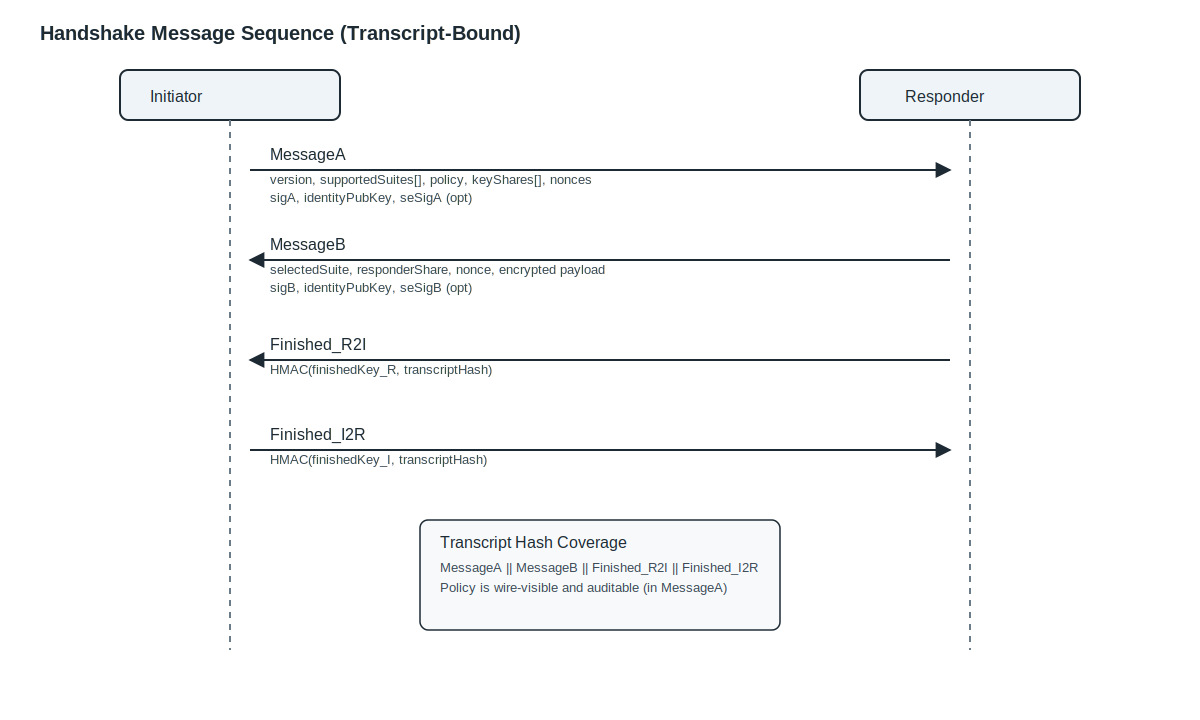
\includegraphics[width=\columnwidth]{_docx_figs/fig_handshake_sequence.png}
\caption{Fig. 1. Handshake sequence with transcript coverage and policy
visibility.}
\label{fig:handshake-sequence}
\end{figure}

MessageA carries the \nbcode{supportedSuites[]} (offered suites) and
\nbcode{keyShares[]} arrays (up to two entries to bound size); MessageB
selects a suite and binds MessageA via \texttt{sigB}. Both sides verify
that the selected suite was offered and that a matching key share
exists, preventing negotiation mismatch. Under the two-attempt strategy
(Section~6.7),
PQC and classic are not co-offered in a single \texttt{MessageA}; when
fallback is permitted, the Initiator retries with a classic-only
\texttt{MessageA} after a whitelist of locally generated capability and
negotiation failures. Explicit key confirmation uses two small Finished
frames to avoid half-open state. Full wire-format definitions, field
validation rules, and encoding rationale appear in the Supplementary
Materials (Wire Format and Validation Rules).

\begin{table*}[!t]
\centering
\noindent\textit{TABLE II. Suite negotiation scenarios under the two-attempt strategy (homogeneous per attempt).}\par
\begin{tabular}{llll}
\hline
Initiator attempt(s)
& Responder Capability
& Outcome
& Notes
\\
\hline
Attempt 1: PQC-only & PQC available & PQC established & Best available selected \\
Attempt 1: PQC-only; Attempt 2: classic-only & Classic only (no PQC material) & Classic established & Graceful fallback (evented) \\
PQC-only (\texttt{strictPQC}) & Classic only & Handshake failed & Policy enforced (no fallback) \\
Classic-only & PQC available & Classic established & Initiator policy respected \\
\hline
\end{tabular}
\end{table*}

\textbf{Failure Semantics:}
\begin{itemize}\tightlist
\item
  All failures trigger \texttt{HandshakeContext.}\\
  \texttt{zeroize()} before error propagation
\item
  Security events are emitted for audit logging
\item
  No partial state is retained after failure
\end{itemize}

\begin{figure*}[!t]
\centering
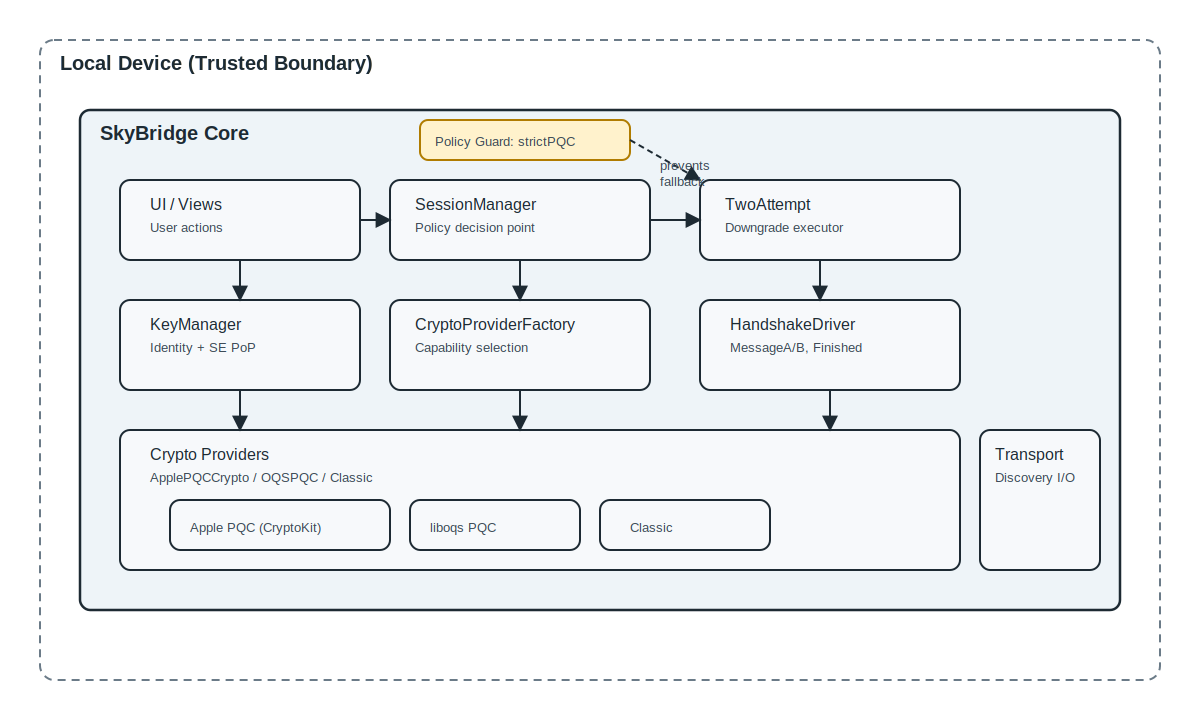
\includegraphics[width=0.95\linewidth]{_docx_figs/fig_architecture.png}
\caption{Fig. 2. SkyBridge Compass system architecture showing device-local trust
boundary (dashed) and policy guard (diamond).}
\label{fig:architecture}
\end{figure*}

\subsection{CryptoProvider
Protocol}\label{b.-cryptoprovider-protocol}

The CryptoProvider protocol defines a unified interface for all
cryptographic operations required by the handshake and session layers [37].
This abstraction enables transparent substitution of underlying
implementations without modifying caller code.


The \texttt{SigningKeyHandle} abstraction resolves the apparent conflict
between ``private key as Data'' and ``Secure Enclave keys never leave
hardware.'' Software keys are one variant; hardware-backed keys use a
reference or callback, ensuring the protocol interface does not assume
exportability.

The protocol mandates \texttt{Sendable} conformance, ensuring
thread-safe usage across Swift's structured concurrency model. Each
provider exposes its tier classification (\texttt{nativePQC},
\texttt{liboqsPQC}, or \texttt{classic}) and active cipher suite,
enabling runtime introspection for logging and policy enforcement.

\subsection{CryptoSuite Wire
Format}\label{c.-cryptosuite-wire-format}

A \textbf{suite} defines the handshake tuple
\texttt{(KEM,\ SIG,\ AEAD,\ KDF)} used for the KEM-DEM envelope and
transcript binding. Data-plane AEAD is negotiated separately and is
fixed to AES-256-GCM in v1 (Table~9). Suite identifiers use a compact
16-bit wire ID with reserved ranges for hybrid, PQC, classic, and
experimental suites to enable forward compatibility. The full range
table, encoding rules, and X-Wing notes appear in the Supplementary
Materials (Suite Identifiers and Wire Format). Unknown suite identifiers
are parsed as \texttt{unknown(wireId)} for audit visibility and forward
compatibility; negotiation rejects unknown values if they appear in
\texttt{keyShares} or as \texttt{selectedSuite}.

\subsection{Provider Factory and
Selection}\label{d.-provider-factory-and-selection}

The \texttt{CryptoProviderFactory} implements deterministic provider
selection based on runtime capability detection and policy
configuration:


The selection algorithm proceeds as follows:

\begin{enumerate}\raggedright
\tightlist
\item
  \textbf{Capability Detection:} Query the environment for native PQC
  availability and liboqs presence.
\item
  \textbf{Policy Application:} Match detected capabilities against the
  requested policy.
\item
  \textbf{Provider Instantiation:} Create the appropriate provider
  instance for the detected environment and policy.
\item
  \textbf{Event Emission:} Emit a \texttt{SecurityEvent} recording the
  selection decision.
\end{enumerate}

{\raggedright
For \texttt{preferPQC} policy, the precedence order is
\texttt{ApplePQCProvider} $\rightarrow$ \texttt{OQSPQCProvider} $\rightarrow$
\texttt{ClassicProvider}. This order is deterministic. The
\texttt{requirePQC} policy returns an \texttt{UnavailablePQCProvider}. It
throws on all operations if no PQC implementation is available.\par}

\textbf{Terminology alignment.}
We use two orthogonal knobs: provider selection
(\texttt{preferPQC}/\texttt{requirePQC}) and handshake fallback policy
(\texttt{default}/\texttt{strictPQC}). In our evaluation, \texttt{default}
corresponds to prefer-PQC with evented classic fallback permitted, while
\texttt{strictPQC} corresponds to requiring PQC and forbidding fallback.

\subsection{KEM-DEM Authenticated Encryption
Format}\label{e.-kem-dem-authenticated-encryption-format}

We use a KEM-DEM envelope (KEM $\rightarrow$ HKDF $\rightarrow$ AEAD) as
a compatibility layer when native HPKE is unavailable, binding role and
transcript into the key schedule with explicit length limits for DoS
protection. On Apple 26+ platforms, we use native CryptoKit PQC
primitives (ML-KEM/ML-DSA) within the same envelope to preserve a single
wire format across platforms. Full header/body formats, versioning, and
length limits are provided in the Supplementary Materials (KEM-DEM
Envelope).



\section{HANDSHAKE STATE
MACHINE}\label{sec:handshake-state-machine}

\subsection{Design Principles}\label{a.-design-principles}

The handshake subsystem addresses three critical requirements:

\begin{enumerate}
\tightlist
\item
  \textbf{Race Condition Prevention:} Concurrent message arrival and
  timeout expiration must not cause double-resume of continuations.
\item
  \textbf{Sensitive Material Protection:} Ephemeral private keys and
  shared secrets must be zeroized on all exit paths.
\item
  \textbf{Observability:} All state transitions and failures must emit
  structured events.
\end{enumerate}

\subsection{Actor-Isolated
Architecture}\label{b.-actor-isolated-architecture}

The \texttt{HandshakeDriver} actor manages handshake state with
compile-time data race prevention:


The \texttt{HandshakeContext} actor isolates sensitive cryptographic
material:


\textbf{Reentrancy Considerations.} Swift actors permit method re-entry
at suspension points (\texttt{await}). While actor isolation prevents
data races, it does not prevent interleaving of method executions. Our
\texttt{HandshakeDriver} mitigates reentrancy risks by routing completion
through \texttt{finishOnce(with:)}, buffering early results, canceling
timeouts on completion, and advancing state before \texttt{await}
points.

\textbf{Await-window limitation.} The
\texttt{handle MessageB} method awaits \texttt{cryptoProvider} operations
inside the actor. If a new message arrives during this await, the actor
could theoretically process it before the current operation completes.
We mitigate this by advancing state to \texttt{.processingMessageB}
before the await, copying immutable inputs, validating a monotonic epoch
counter after resumption, and emitting security events on unexpected
transitions.

This approach provides structural protection against reentrancy hazards
rather than relying on timing assumptions. A formal analysis using model
checking is planned for future work.

\subsection{State Transitions}\label{c.-state-transitions}

Fig.~3 illustrates the handshake state machine for both roles.

\begin{figure}[!t]
\centering
\includegraphics[width=0.95\linewidth]{_docx_figs/fig_state_machines.png}
\caption{Fig. 3. Handshake state machines for Initiator (top) and Responder
(bottom).}
\label{fig:state-machines}
\end{figure}

\subsection{Double-Resume
Prevention}\label{d.-double-resume-prevention}

The \texttt{finishOnce} method provides a single convergence point for handshake completion, handling the race between timeout expiration and message arrival by: (1) canceling the timeout task on any completion, (2) guarding continuation access with immediate nil assignment, and (3) buffering early results for late continuation establishment.

\subsection{Secure Zeroization}\label{e.-secure-zeroization}

Swift's standard \texttt{Data} and \texttt{Array} types use copy-on-write (COW) semantics, which can leave uncontrolled copies of sensitive material in memory. The \texttt{SecureBytes} class addresses this by using manual \texttt{UnsafeMutableRawPointer} allocation to maintain exclusive ownership, preventing COW-induced secret proliferation. All failure paths explicitly call \texttt{context.zeroize()} before error propagation, with \texttt{deinit} zeroization as defense-in-depth. On Darwin platforms, zeroization uses platform-supported secure wipe primitives (e.g., \texttt{explicit_bzero} or \texttt{memset_s}) where available. We avoid exporting secrets as \texttt{Data} when possible, but acknowledge that OS-level snapshots, API boundary copies, or privileged inspection can still retain residues; zeroization is a defense-in-depth measure rather than a sole security boundary.

\subsection{Transcript Binding and Signature
Separation}\label{f.-transcript-binding-and-signature-separation}

The protocol uses domain-separated signatures to prevent cross-message
and cross-session replay attacks.

\textbf{Signature A (MessageA)} is computed by the Initiator over the
MessageA-local fields, binding suite preference, policy intent, and
identity context before any responder data is received:

Signature A preimage includes the domain separator \texttt{SkyBridge-A},
the version, canonical supported suites and key shares, the client nonce,
capabilities, policy, and the initiator identity public key; optional
Secure Enclave binding uses \texttt{SkyBridge-SE-A}.

\textbf{Signature B (MessageB):} The Responder signs a transcript that
commits to MessageA:

Signature B preimage includes the domain separator \texttt{SkyBridge-B}
plus \texttt{transcriptA}, selected suite wire ID, responder key share,
server nonce, payload hash, and the responder identity public key;
optional Secure Enclave binding uses \texttt{SkyBridge-SE-B}.

\textbf{Key Derivation:} Nonces, transcripts, suite binding, and
\emph{directional separation} are included in the KDF, and the salt is
transcript-bound (non-empty):

KDF input concatenates the \texttt{SkyBridge-KDF} label, suite wire ID,
transcript hashes, and nonces. The salt uses the domain string
\texttt{SkyBridge-KDF-Salt-v1|}. Direction labels separate traffic
classes:
\begin{itemize}
\item \texttt{initiator_to_responder}
\item \texttt{responder_to_initiator}
\end{itemize}


This structure is designed to ensure: (1) \texttt{sigB} commits to \texttt{MessageA},
so any tampering breaks verification; (2) domain separators prevent
cross-protocol attacks; (3) SE signatures are session-bound and
non-replayable.



\section{SECURITY MODEL AND
GUARANTEES}\label{sec:security-model}

\subsection{Security Model}\label{a.-security-model}

We assume an active network adversary with full control of the discovery
channel (drop, delay, reorder, duplicate, modify, and inject messages)
but without breaking standard cryptographic assumptions. The attacker
can replay prior handshakes and attempt downgrade by suppressing
PQC-related fields. We assume the out-of-band pairing ceremony is
trusted and that device key storage (Keychain/Secure Enclave) preserves
key integrity. The attacker may compromise a peer after pairing and
learn long-term signing key material, but cannot retroactively forge
signatures for past sessions. We do not claim forward secrecy for
KEM-based suites in v1: ML-KEM encapsulation targets a peer's long-term
KEM public key obtained during pairing. Accordingly, post-quantum
confidentiality against store-now-decrypt-later adversaries holds only
while long-term KEM private keys remain uncompromised; later compromise
of the corresponding KEM private key can enable decryption of recorded
sessions.

\textbf{Assumptions:}
\begin{itemize}\tightlist
\item
  The pairing ceremony delivers the correct peer identity key (PIN or
  visual verification is not bypassed).
\item
  Pinned identity keys stored in Keychain/Secure Enclave retain integrity
  across normal device operation.
\item
  Devices remain uncompromised (no root or malware control) during
  handshake execution.
\end{itemize}

\textbf{If assumptions fail:}
\begin{itemize}\tightlist
\item
  If pairing is subverted and the pinned identity key is replaced,
  peer authentication is no longer meaningful; the system must require
  re-pairing and treat the session as untrusted.
\item
  If device integrity is lost, confidentiality and key secrecy cannot be
  guaranteed; the system should abort and emit high-severity events such
  as \texttt{identity}\texttt{Mismatch} or
  \texttt{handshake}\texttt{Failed}.
\end{itemize}

\subsection{Security Goals and Proof
Sketches}\label{b.-security-goals-and-proof-sketches}

\textbf{Definitions.}
\begin{itemize}\tightlist
\item \textbf{D1 (Forced downgrade / forced fallback).} A downgrade occurs if a session is established with a classic suite when policy requires PQC (\texttt{strictPQC}), or if classic fallback is accepted under the default policy without satisfying the local-only fallback gate (Definition D2) and without emitting the corresponding audit event (Property G8).
\item \textbf{D2 (Local-only fallback gate).} Fallback is permitted only after (i) the peer identity is verified against the pinned key (paired peers) and (ii) the triggering failure is locally generated capability/instantiation unavailability (whitelist), excluding timeout and any unauthenticated network-derived failure.
\item \textbf{D3 (Audit evidence).} The minimal sufficient evidence set is the tuple \{event type, timestamp, deviceId, suiteId, failure reason code, policy mode, fallback flag, cooldown remaining\} (Property G8).
\end{itemize}

We state the core properties as invariants and provide non-formal proof
sketches tied to protocol mechanics. Formal verification using model checking or symbolic analysis [29] is planned for future work:

\textbf{Property G1 (Negotiation Integrity):} The selected suite must be
among the Initiator's offered suites and have a corresponding key
share.\\
\emph{Proof sketch:}
\begin{itemize}\tightlist
\item
  \texttt{MessageB} includes \texttt{selectedSuite}, and
  \texttt{sigB} covers \texttt{MessageA}.
\item
  Any modification to the offered suite list or key-share list breaks
  \texttt{sigB} verification.
\item
  The Responder validates \texttt{selectedSuite} against the offered
  suites and checks that a matching key share is present.
\end{itemize}

\textbf{Property G2 (Mutual Authentication for Paired Peers):} For
previously paired devices, the peer identity is authenticated and bound
to the handshake transcript.\\
\emph{Proof sketch:}
\begin{itemize}\tightlist
\item
  \texttt{identityPubKey} is pinned during OOB pairing.
\item
  \texttt{MessageA}/\texttt{MessageB} signatures over transcript data
  must verify under the pinned key; otherwise
  \texttt{identityMismatch} aborts the handshake.
\end{itemize}

\textbf{Property G3 (Session Key Secrecy):} The derived session keys
remain secret under standard KEM/DH and signature security
assumptions.\\
\emph{Proof sketch:}
\begin{itemize}\tightlist
\item
  The shared secret is derived from KEM decapsulation or DH, and keys
  are extracted via HKDF with transcript-bound salt.
\item
  An attacker without the private key material cannot compute the shared
  secret or derive session keys.
\end{itemize}

\textbf{Property G4 (Replay Resistance):} Replayed handshakes do not
establish a session.\\
\emph{Proof sketch:} \texttt{handshakeId} derives from fresh nonces and
suite identifiers; replay detection caches recent IDs and rejects
duplicates within the window.

\textbf{Property G5 (Downgrade Resistance under strictPQC):} No fallback
to classic is allowed under strict policy.\\
\emph{Proof sketch:} \texttt{TwoAttemptHandshakeManager} enforces a
policy gate before any fallback attempt; strictPQC forbids all fallback
edges regardless of error type. This is validated by policy downgrade
benchmarks (Fig.~4).

\textbf{Property G6 (Safe Fallback under default policy):} Fallback can
only occur after peer identity is verified under the pinned key and only
for a whitelisted set of locally generated capability errors; timeout
and network-derived failures never trigger fallback.\\
\emph{Proof sketch:} Fallback is gated after identity verification; the
whitelist is evaluated on locally generated capability/instantiation
errors rather than unauthenticated network input. \texttt{timeout} is
explicitly blocked and per-peer cooldown limits repeated downgrades.
\emph{Proposition (No forced fallback by packet loss):} Under the attacker model in Section~5, an active network attacker who can drop/delay/reorder messages cannot induce a successful classic session by causing timeouts, because timeout-triggered fallback is disallowed and the default-policy fallback gate (Definition D2) requires locally generated unavailability after identity verification.

\textbf{Property G7 (Legacy Acceptance Preconditions):} Legacy P-256
signatures are accepted only under authenticated pairing or an existing
trust record.\\
\emph{Proof sketch:} Legacy acceptance is gated by
\texttt{Legacy Trust Precondition}; pure network stranger connections fail.
This is validated by the precondition test matrix (Table~6).

\textbf{Property G8 (Auditability):} Cryptographic downgrades and
exceptional states are observable via a minimal sufficient information set.\\
\emph{Proof sketch:} The handshake emits
\texttt{cryptoDowngrade} events with reason,
deviceId, and cooldown context, enabling post-hoc verification of policy
adherence.

\emph{Audit field requirements:}
\begin{itemize}\tightlist
\item \textbf{MUST log} (minimal sufficient set): event type, timestamp, deviceId, suiteId, failure reason code, policy mode, fallback triggered (bool), cooldown remaining.
\item \textbf{MUST NOT log} (privacy preservation): session keys, nonces, raw signatures, message payloads, user identifiers beyond deviceId.
\item \textbf{Tamper-evidence:} Events are emitted synchronously before state transitions complete; the resulting trace is checkable against expected state-machine templates (used in our audit-signal fidelity tests). Log collection relies on OS unified logging (\texttt{os_log}) for best-effort retention and is not a cryptographic tamper-proof store; privileged adversaries can alter or truncate logs.
\end{itemize}

\begin{table*}[!t]
\centering
\noindent\textit{TABLE III. Security Contract (Properties, Enforcement, Evidence).}\par
\begin{tabular}{lll}
\hline
Property
& Enforced at
& Evidence
\\
\hline
G1 Negotiation integrity & Suite/keyshare validation + transcript-bound \texttt{sigB} & Fig.~1, \mbox{HandshakeDriverTests} \\
G2 Mutual authentication & Identity pinning + signature verification & Table~5 (wrong signature), Table~6 \\
G3 Session key secrecy & KEM/DH + HKDF with transcript-bound salt & Property 1, Supplementary Materials (ML-DSA Key Sizes) \\
G4 Replay resistance & \texttt{handshakeId} cache + nonce binding & Property-Oriented Testing (Section~7) \\
G5 strictPQC no-downgrade & Policy gate in TwoAttemptHandshakeManager & Fig.~4, \mbox{PolicyDowngradeBenchTests} \\
G6 Default safe fallback & Whitelist/blacklist + local capability gate + cooldown & Fig.~5, Table~5 \\
G7 Legacy acceptance precondition & LegacyTrustPrecondition & Table~6 \\
G8 Auditability & Security event emission & Fig.~6, Table~7 \\
\hline
\end{tabular}
\end{table*}



\section{Implementation}\label{sec:implementation}

Implementation references (source files, line numbers) are consolidated in the Supplementary Materials (Artifact Map).

\subsection{Platform Support
Matrix}\label{a.-platform-support-matrix}

SkyBridge Compass uses a tiered provider model: a native PQC provider
when available (e.g., CryptoKit ML-KEM/ML-DSA), a portable liboqs
provider, and a classic provider. Provider selection is deterministic
and prefers the strongest available tier; Secure Enclave proof-of-
possession is optional and orthogonal to the negotiated suite. The full
platform support matrix and suite availability are in the Supplementary
Materials (Platform Support Matrix).

\subsection{Native PQC Integration}\label{b.-apple-pqc-integration}

The native provider wraps CryptoKit ML-KEM/ML-DSA APIs [1] when the
SDK exposes them, enabling platform-backed PQC suites and HPKE-based
encapsulation. We treat this as a deployment instance rather than a
protocol dependency; integration details are provided in the
Supplementary Materials (Native PQC Integration).

\subsection{Conditional Compilation
Strategy}\label{c.-conditional-compilation-strategy}

PQC symbols are gated behind build-time flags to keep the codebase
buildable on SDKs that lack PQC types and to avoid compile-time
failures. The flagging strategy and build settings are detailed in the
Supplementary Materials (Conditional Compilation).

\subsection{Security Event
Emission}\label{d.-security-event-emission}

All cryptographic decisions emit structured events for auditability.
The emitter provides backpressure and rate limiting; implementation
details are in the Supplementary Materials (Security Event Emission).

\subsection{Secure Enclave
Integration}\label{e.-secure-enclave-integration}

For hardware-backed signing, a \texttt{SigningCallback} protocol allows
Secure Enclave keys without exposing private material. Availability,
fallback behavior, and key-type details are provided in the
Supplementary Materials (Secure Enclave Integration).

\subsection{Signing Key Hierarchy}\label{f.-signing-key-hierarchy}

The system uses two complementary signatures: (1) protocol signatures
via the negotiated suite (Ed25519 for classic, ML-DSA-65 for PQC) to bind
peer identity to the transcript, and (2) optional Secure Enclave
P-256 signatures for device proof-of-possession. Protocol signatures are
mandatory; Secure Enclave PoP is optional and provides a hardware-backed
signal. Key hierarchy details and verification rules are provided in the
Supplementary Materials (Signing Key Hierarchy).

\subsection{Pre-Negotiation Signature Algorithm Selection and
Two-Attempt
Strategy}\label{g.-pre-negotiation-signature-algorithm-selection-and-two-attempt-strategy}

A fundamental challenge is that \texttt{sigA} must be generated before
negotiation completes, yet the signature algorithm should match the
negotiated suite. We resolve this with pre-negotiation signature
selection and a two-attempt strategy. Each attempt is homogeneous
(PQC-only or classic-only), and the signature algorithm is chosen based
on the offered suites. The initiator first attempts PQC, then falls back
to classic only for a whitelist of benign, locally generated capability
errors after peer identity verification; timeout, signature
verification, identity mismatch, replay, and other network-derived
failures never trigger fallback. This policy is enforced by the
handshake manager and logged as security events. Detailed error lists
and type-level enforcement are provided in the Supplementary Materials
(Two-Attempt Strategy).

\textbf{Fallback Boundary Conditions (Explicit Scope):}
\begin{itemize}\tightlist
\item \emph{We defend against:} (1) Attacker-induced timeout forcing downgrade (blocked by timeout blacklist); (2) Rapid downgrade cycling via repeated failures (5-minute per-peer cooldown); (3) Signature/identity attacks masquerading as capability failures (verification failures are blacklisted).
\item \emph{We do not defend against:} (1) Attacker persistently blocking PQC traffic for $>$5 minutes (availability vs.\ security trade-off; strictPQC mode provides full protection at cost of connectivity); (2) Legitimate PQC provider failures causing temporary classic fallback (by design, to maintain usability).
\item \emph{Cooldown rationale:} We set a conservative default of 5 minutes to bound downgrade cycling while limiting availability impact; the cooldown is a tunable policy knob, and strictPQC users requiring zero-downgrade guarantees should disable fallback entirely.
\end{itemize}

\textbf{Attempt State and Identifiability:}
\begin{itemize}\tightlist
\item \emph{Shared across attempts:} pinned identity fingerprint and pinned KEM public keys (trust record), and per-peer fallback cooldown state.
\item \emph{Not shared across attempts:} nonces, transcript hashes, handshakeId/replay tags, ephemeral key shares, and session keys; each attempt runs a fresh state machine.
\item \emph{Identifiability:} a passive observer can distinguish a classic fallback attempt from a PQC attempt by wire format. We do not transmit an explicit attempt counter, and strictPQC disables fallback when capability privacy outweighs compatibility.
\end{itemize}

\textbf{Security Events:}

Every fallback emits a \texttt{cryptoDowngrade} event with full
context (reason, deviceId, cooldown), enabling audit and anomaly
detection.



\section{Evaluation}\label{sec:evaluation}

\subsection{Experimental Setup}\label{a.-experimental-setup}

We evaluate SkyBridge Compass along two primary tracks:
\textbf{security-centric evidence} (fault injection, downgrade
suppression, legacy precondition enforcement, and auditability) and
\textbf{cost-centric evidence} (handshake latency, wire overhead,
provider selection overhead, and data-plane throughput).

\textbf{Environment:} All experiments are run on Apple Silicon (M1/M3 class) with macOS 26.x, where CryptoKit PQC is available when the SDK exposes ML-KEM/ML-DSA types. Build configuration uses Release (\texttt{-O}) with non-essential logging disabled. Timing uses a monotonic clock (\texttt{ContinuousClock}) with N=1000 iterations after 10 warmup runs; reported percentiles (p50/p95/p99) are computed directly from samples.

\textbf{Repeatability:} For each configuration, we run 3--5 independent
batches by restarting the benchmark test process; Supplementary
Tables~S5--S6
report mean and 95\% confidence intervals across batches.

\textbf{Reproducibility:} We ship an opt-in benchmark suite under \texttt{Tests/SkyBridgeCoreTests/}. For a one-shot run, use \texttt{Scripts/run_paper_eval.sh}. The complete command reference and CSV artifact specifications are provided in the Supplementary Materials (Reproducibility).

\textbf{iOS Reproducibility:} Because CI-style automation for iOS PQC
measurements is sensitive to device availability and simulator runtime
support, we also ship an on-device micro-benchmark in the iOS app that
exports JSON artifacts (timestamped) for Supplementary tables. This
enables independent reproduction of KEM, signature, and KEM--DEM costs on
commodity iOS 26+ hardware without modifying the protocol code paths.

\begin{table*}[!t]
\centering
{\setlength{\tabcolsep}{3pt}\small
\noindent\textit{TABLE IV. On-device micro-benchmark on iOS 26.2 (iPhone, N=50). Metrics are reported in milliseconds (ms) as mean and p99 over 50 iterations (no warmup). Artifacts are exported as JSON (schema v2) and include split suite labels (\texttt{kem_suite}, \texttt{sig_suite}) for academic clarity. Each ``encapsulate'' measurement includes the sender-side ephemeral generation and encapsulation work for the corresponding KEM/key-agreement.}\par
\begin{tabular}{lllll}
\hline
Configuration &
KEM encaps.\newline(mean/p99) &
Sign\newline(mean/p99) &
Verify\newline(mean/p99) &
\shortstack[l]{KEM--DEM\\seal+open\\(mean/p99)} \\
\hline
Classic (X25519 + Ed25519) & 0.414 / 0.704 & 0.122 / 0.126 & 0.085 / 0.133 & 0.389 / 0.534 \\
CryptoKit PQC (ML-KEM-768 + ML-DSA-65) & 0.149 / 0.190 & 1.072 / 2.108 & 0.048 / 0.055 & 0.245 / 0.272 \\
CryptoKit Hybrid (X-Wing + ML-DSA-65) & 0.282 / 0.452 & 1.403 / 2.654 & 0.048 / 0.053 & 0.324 / 0.391 \\
\hline
\end{tabular}
}
\end{table*}

\textbf{Interpretation:} The loopback microbench isolates cryptographic and state-machine overhead; it does not model OS network stacks, NAT traversal, or heterogeneous access networks. We report simulated impairments separately (Section~7.4) and list real-network end-to-end measurement as future work (Section~8).

\subsection{Security Validation}\label{b.-security-centric-evaluation}

We validate security properties through fault injection, property-based
testing, and audit-signal fidelity analysis. This section presents the
key results; detailed test matrices and methodology are provided in the
Supplementary Materials (Regression Testing).

\textbf{Failure-Mode Robustness.}
The actor-isolated handshake driver provides deterministic failure semantics without unhandled errors, double-resume, or sensitive-material leaks. We inject faults including timeout, malformed framing, invalid signatures, out-of-order delivery, and concurrent cancellation (n=1000 per scenario per policy).

\textbf{Unknown-suite handling:} We parse unknown suite identifiers as an
explicit \texttt{unknown(wireId)} value and reject them if they appear in
\texttt{keyShares} or as \texttt{selectedSuite}. This prevents silent
``unknown $\rightarrow$ classic'' coercions that would otherwise weaken
downgrade guarantees.

\begin{table*}[!t]
\centering
\noindent\textit{TABLE V. Failure-Mode Robustness and Observability. Runs = number of
iterations per scenario and policy (n=1000). Table reports default
policy; strictPQC counts are recorded separately in
\texttt{fault_injection_2026-01-16.csv}. All
metrics are binary (1 = pass) except event counts. Data from
\texttt{Artifacts/fault_injection_2026-01-16.csv}
produced by \mbox{HandshakeFaultInjectionBenchTests}; semantic checks from
\mbox{HandshakeDriverTests}.}\par
\begin{tabular}{lllllll}
\hline
Failure Mode
& Runs
& No\\Unexp.\\Error
& No\\Double\\Resume
& Zero\\Verified
& $E_{\texttt{handshakeFailed}}$
& $E_{\texttt{cryptoDowngrade}}$
\\
\hline
Out-of-order & 1000 & 1 & 1 & 1 & 0 & 0 \\
Duplicate & 1000 & 1 & 1 & 1 & 0 & 0 \\
Drop & 1000 & 1 & 1 & 1 & 1000 & 0 \\
Delay within timeout & 1000 & 1 & 1 & 1 & 0 & 0 \\
Delay exceed timeout & 1000 & 1 & 1 & 1 & 1000 & 0 \\
Corrupt header & 1000 & 1 & 1 & 1 & 1000 & 0 \\
Corrupt payload & 1000 & 1 & 1 & 1 & 1000 & 0 \\
Wrong signature & 1000 & 1 & 1 & 1 & 1000 & 0 \\
Concurrent cancel & 1000 & 1 & 1 & 1 & 1000 & 0 \\
Concurrent timeout & 1000 & 1 & 1 & 1 & 1000 & 0 \\
\hline
\end{tabular}
\end{table*}

The delay-within-timeout and delay-exceed-timeout scenarios approximate
RTT jitter and loss-induced stalls, while drop and duplicate cases
approximate packet loss and reordering. The per-scenario event
distributions are recorded in \texttt{Artifacts/fault_injection_2026-01-16.csv}.

Downgrade events are quantified separately in the policy bench (Fig.~4)
to avoid conflating fallback behavior with transport corruption
scenarios.

\begin{figure}
\centering
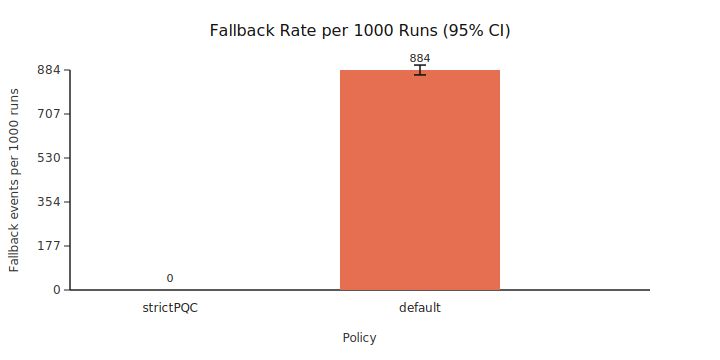
\includegraphics[keepaspectratio,width=\columnwidth]{_docx_figs/fig_policy_downgrade.png}
\caption{Fig. 4. Policy guard enforces strictPQC: fallback events per
1000 runs, macOS 26.x, N=1000 per policy. Error bars show 95\% Wilson binomial CI.}
\label{fig:policy-downgrade}
\end{figure}

The plot in Fig.~4 uses the policy-downgrade
dataset. File: \texttt{policy_downgrade_2026-01-16.csv}. It
demonstrates that strictPQC never emits fallback events even under
forced PQC-unavailable errors; default policy shows non-zero downgrade
events.

\begin{figure}
\centering
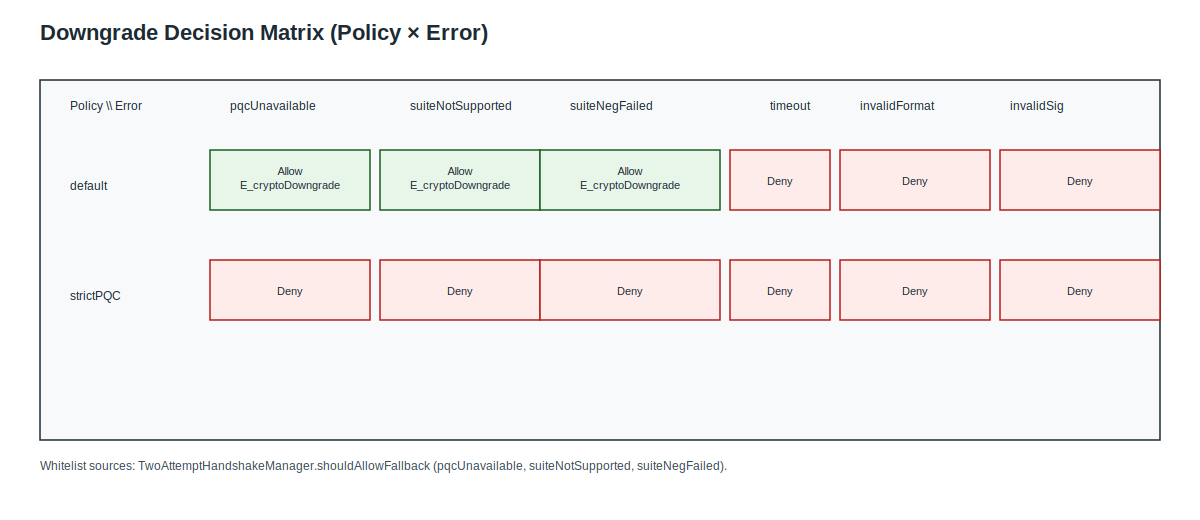
\includegraphics[keepaspectratio,width=\columnwidth]{_docx_figs/fig_downgrade_matrix.png}
\caption{Fig. 5. Downgrade decision matrix (policy × error) with
explicit allow/deny semantics, macOS 26.x. Each cell is labeled ALLOW or DENY for grayscale readability.}
\label{fig:downgrade-matrix}
\end{figure}

Fig.~5 encodes the explicit downgrade whitelist/blacklist: only
PQC-unavailability and suite-selection errors may fallback under default
policy; strictPQC denies all fallback edges.

\begin{figure}
\centering
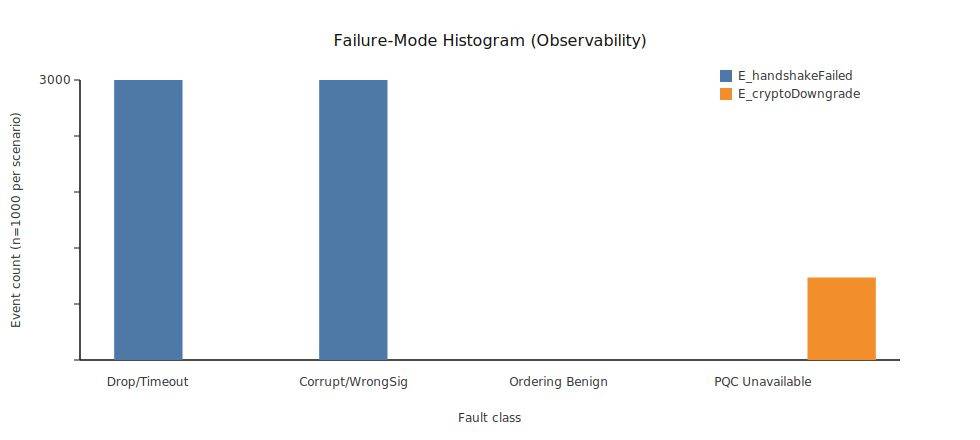
\includegraphics[keepaspectratio,width=\columnwidth]{_docx_figs/fig_failure_histogram.png}
\caption{Fig. 6. Failure-mode histogram of security events, macOS 26.x,
N=1000 per scenario.}
\label{fig:failure-histogram}
\end{figure}

Fig.~6 combines fault-injection counts with the downgrade-acceptance
event from the policy bench to visualize observability of failures and
downgrades across policy modes.

\textbf{\mbox{Property-Oriented} Testing.}
Correctness properties are validated with property-based tests using reproducible seeds (0xDEADBEEF). Key properties include: (1) KEM-DEM round-trip correctness across all providers (100 trials), (2) signature verification integrity (100 payloads per provider), (3) secure zeroization on deallocation, and (4) state-machine single-resume guarantee under concurrent stress (500 iterations). A standalone Python decoder (\texttt{Scripts/wire_format_sanity.py}) provides non-Swift interoperability validation of wire formats.

\textbf{ML-DSA Key Lifecycle.}
ML-DSA-65 key generation, storage, and sign-verify operations are
validated against FIPS 204 specifications [16]. Size compliance
results are reported in the Supplementary Materials (ML-DSA Key Sizes);
all property tests (round-trip, tampering detection, key independence)
achieve 100\% pass rate. Keys are stored in Keychain with
\texttt{kSecAttrAccessible AfterFirstUnlock ThisDeviceOnly}
and \texttt{kSecAttrSynchronizable= false} to ensure
device-local protection.

\textbf{Legacy Fallback Security.}
Legacy P-256 signatures are only accepted when a security precondition is satisfied: (1) authenticated out-of-band channel (QR code, PAKE/PIN), or (2) existing TrustRecord with \texttt{legacyP256PublicKey}. Pure network stranger connections are rejected to prevent downgrade attacks.

\begin{table*}[!t]
\centering
\noindent\textit{TABLE VI. Legacy Fallback Precondition Test Results. All tests executed
via \mbox{LegacyFallbackPreconditionTests}. Tests validate Property 7: Legacy
Fallback Security Precondition.}\par
\begin{tabular}{llll}
\hline
Scenario
& Precondition
& Expected Result
& Actual Result
\\
\hline
Pure network stranger & None & Reject & OK Reject \\
QR code pairing (verified) & authenticatedChannel & Allow & OK Allow \\
PAKE pairing (verified) & authenticatedChannel & Allow & OK Allow \\
Existing TrustRecord with legacy key & existingTrustRecord & Allow & OK Allow \\
Existing TrustRecord without legacy key & None & Reject & OK Reject \\
Network discovery & None & Reject & OK Reject \\
Unverified authenticated channel & None & Reject & OK Reject \\
\hline
\end{tabular}
\end{table*}

\textbf{Property 7 (Legacy Fallback Security Precondition):} A legacy
P-256 signature SHALL only be accepted when a security precondition is
satisfied. Pure network stranger connections SHALL be rejected.
Validated with 12 test cases covering all precondition combinations (100\% coverage of the precondition state space).

\textbf{Audit-Signal Fidelity.}
Security events provide deterministic, audit-friendly (best-effort, non-cryptographic) telemetry of failures and policy decisions. Fig.~7 illustrates a representative timeout trace showing attacker action, policy gate response, and emitted event.

\emph{Evaluation approach:} We evaluate audit-signal fidelity using a spec-to-event mapping consistency metric, \emph{not} a statistical classifier. Each fault-injection scenario deterministically maps to exactly one expected trace template (event sequence), e.g., timeout $\rightarrow$ \texttt{handshakeFailed=1, cryptoDowngrade=0}. Match rate (MR)=1.00 means all N iterations matched the expected template; spurious rate (SR)=0.00 means no unexpected events were emitted. This is regression consistency against the protocol specification, not ML classification performance.

Table~7 summarizes results across all fault-injection scenarios: all scenario classes achieve 1.00 match and 0.00 spurious rates, confirming correct event semantics.

\begin{figure}
\centering
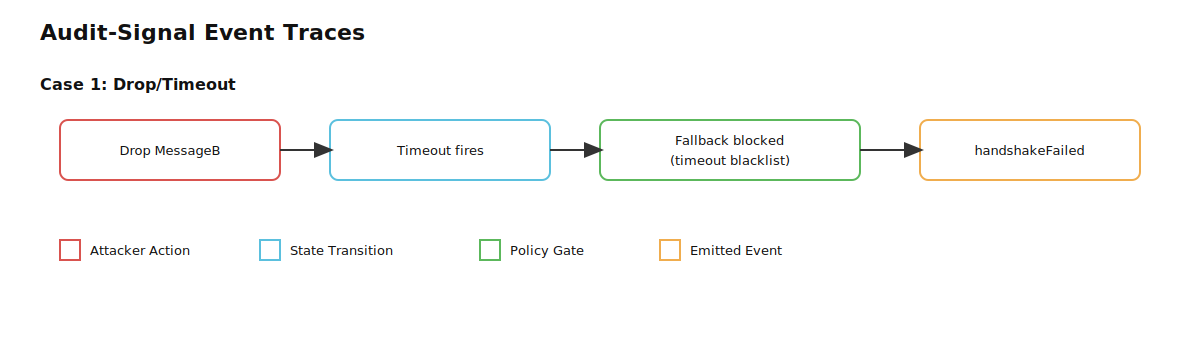
\includegraphics[keepaspectratio,width=\columnwidth]{_docx_figs/fig_event_traces.png}
\caption{Fig. 7. Audit-signal event trace (representative timeout case)
showing attacker action, policy gate, and emitted event.}
\label{fig:event-traces}
\end{figure}

\begin{table*}[!t]
\centering
\noindent\textit{TABLE VII. Audit-Signal Fidelity Summary. Match/spurious rates reflect \emph{deterministic} protocol event mapping (each scenario maps to exactly one expected trace template), not statistical classification. Perfect scores indicate regression consistency against the protocol specification.}\par
\begin{tabular}{lllll}
\hline
Scenario Class & Expected Signal & N & Match (MR) & Spurious (SR) \\
\hline
Drop/Timeout (default) & handshakeFailed=1, cryptoDowngrade=0 & 3000 & 1.00 & 0.00 \\
Drop/Timeout (strictPQC) & handshakeFailed=1, cryptoDowngrade=0 & 3000 & 1.00 & 0.00 \\
Corrupt/Wrong Sig & handshakeFailed=1, cryptoDowngrade=0 & 6000 & 1.00 & 0.00 \\
Ordering Benign & handshakeFailed=0, cryptoDowngrade=0 & 6000 & 1.00 & 0.00 \\
PQC unavailable (default) & cryptoDowngrade=1 & 1000 & 1.00 & 0.00 \\
PQC unavailable (strictPQC) & cryptoDowngrade=0 & 1000 & 1.00 & 0.00 \\
\hline
\end{tabular}
\end{table*}

Due to space constraints, the complete regression test matrix, TLV encoding validation, and implementation component details are provided in the Supplementary Materials (Regression Testing and Artifact Map).

\subsection{Performance Benchmarks}\label{c.-cost-centric-evaluation}

Table~8 consolidates all performance metrics. We measure \mbox{end-to-end} handshake completion time using an in-memory loopback transport to isolate cryptographic and state-machine overhead. Each configuration reports distributional statistics over N=1000 iterations after 10 warmup runs.

% Auto-generated by make_tables.py on 2026-01-16T17:12:20.762559
% DO NOT EDIT MANUALLY - regenerate from CSV artifacts

\begin{table*}[!t]
\centering
\noindent\textit{TABLE VIII. Performance Summary. All benchmarks on Apple Silicon (M1/M3), macOS 26.x, N=1000 iterations after 10 warmup runs. Wire Size counts payload-only handshake bytes (MessageA + MessageB + 2×Finished); loopback wire sizes including transport overhead are reported separately in Table~1 and Supplementary Table~S4. Data-plane AEAD is fixed to AES-256-GCM in v1, so throughput is independent of the negotiated handshake suite; throughput measured post-handshake on 1~MiB payloads.}\par
\begin{tabular}{lllllll}
\hline
Configuration & µlticolumn{2}{c}{Handshake Latency} & µlticolumn{2}{c}{RTT} & Wire Size & Throughput \\
\cmidrule(lr){2-3} \cmidrule(lr){4-5}
 & mean (ms) & p95 (ms) & p50 (ms) & p95 (ms) & (bytes) & (GB/s) \\
\hline
Classic & 1.62 & 1.81 & 0.41 & 0.46 & 827 & 3.7 \\
liboqs PQC & 2.29 & 3.01 & 0.80 & 1.35 & 12,163 & 3.7 \\
CryptoKit PQC & 5.76 & 6.71 & 1.59 & 2.27 & 12,163 & 3.7 \\
\hline
\end{tabular}
\end{table*}

\textbf{Latency Distribution.}
Fig.~8 shows latency percentiles across
configurations. Classic handshakes remain under 2~ms at p99; CryptoKit
PQC stays under 6.4~ms at p99 with variance dominated by ML-DSA signature
verification overhead. Extended statistics (mean/p50/p95/p99, std) are
available in Supplementary Tables~S1--S2
(submitted as separate file \texttt{supplementary.pdf}).

\begin{figure}
{\centering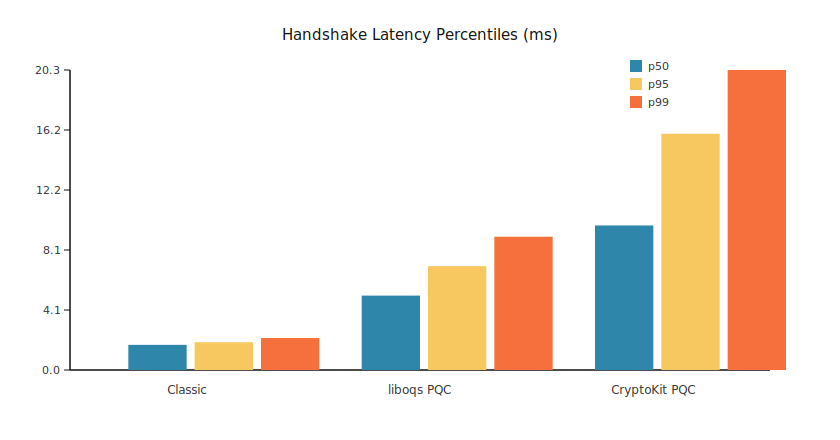
\includegraphics[keepaspectratio,width=\columnwidth]{_docx_figs/fig_handshake_latency.png}\par}
\caption{Fig. 8. Handshake latency percentiles for Classic vs liboqs PQC vs CryptoKit PQC (N=1000). Generated from \texttt{Artifacts/handshake_bench_2026-01-16.csv}; values match the Performance Summary (Table~8) and Supplementary Table~S1.}
\label{fig:handshake-latency}
\end{figure}

\textbf{Wire-Format Breakdown.}
The 15× size increase from Classic (827~B) to PQC (12.2~KB) is dominated by ML-DSA signatures (3309~B) and ML-KEM ciphertexts (1088~B). Fig.~9 shows the per-field breakdown.

\begin{figure}
{\centering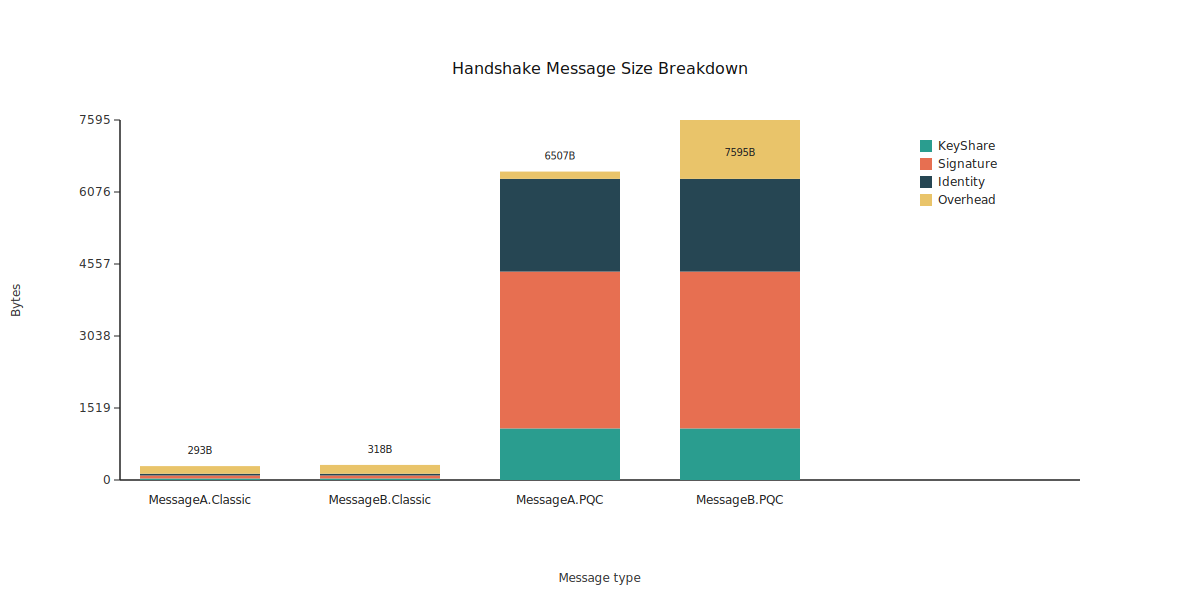
\includegraphics[keepaspectratio,width=\columnwidth]{_docx_figs/fig_message_size_breakdown.png}\par}
\caption{Fig. 9. Handshake message size breakdown (signature, keyshare,
identity fields, framing overhead) for MessageA/MessageB across Classic, PQC (liboqs), and PQC (CryptoKit) configurations. Counts reflect MessageA/B payloads only; the \emph{payload-only} handshake size adds two 38~B Finished frames (accounted for in Table~8), and detailed field sizes are reported in Supplementary Table~S3. Generated from \texttt{Artifacts/message_sizes_2026-01-16.csv}.}
\label{fig:message-size-breakdown}
\end{figure}

Note: X-Wing hybrid KEM adds 32~B to MessageA's keyshare (1120~B vs 1088~B for ML-KEM-768), yielding a measured total handshake size of 12,195~B; detailed field breakdowns are available in Supplementary Table~S3 (\texttt{MessageA.XWing}/\texttt{MessageB.XWing}).

\textbf{Data-Plane and Provider Selection.}
Post-handshake symmetric AEAD (AES-256-GCM) throughput reaches 3.7~GB/s for 1~MB payloads on Apple Silicon, with CPU cost of 0.25~ns/byte. In v1 the data-plane AEAD is fixed to AES-256-GCM and recorded separately from the handshake suite; thus throughput is independent of the negotiated KEM/signature suite. Provider selection overhead is sub-microsecond for cached paths (0.17~µs p50) and under 6~µs even for fallback scenarios. Detailed breakdowns are provided in the artifact CSV files.

\begin{table}[!t]
\centering
\footnotesize
\noindent\textit{TABLE IX. Handshake vs data-plane AEAD selection (v1).}\par
\begin{tabular}{lll}
\hline
Layer & AEAD & Negotiation source \\
\hline
Handshake payloads & AES-256-GCM & Suite tuple \\
Data-plane traffic & AES-256-GCM & Fixed (v1) \\
\hline
\end{tabular}
\end{table}

\subsection{External Validity Under Network Impairments}\label{sec:network-conditions}

We simulate four network conditions with a retry-aware model (max 2
retries) to approximate loss, jitter, and reordering. The simulator is
in-process (not kernel \texttt{netem}): loss is independent Bernoulli per
packet; jitter is sampled uniformly from $\pm$J~ms around base RTT; and
reordering is modeled as an added random delay (50--150~ms) applied to
10\% of packets. Table~10
summarizes completion and p95 latency ranges across classic/liboqs/
CryptoKit suites using \texttt{Artifacts/network_condition_2026-01-11.csv}
generated by \texttt{Scripts/run_network_bench_retry.swift}. Even under severe loss, completion
remains above 99.8\%, and \texttt{handshakeFailed} events track the few
failures; no downgrade events occur because fallback is only permitted
for PQC-unavailability (Fig.~4).

\begin{table*}[!t]
\centering
\noindent\textit{TABLE X. Simulated network impairment results (N=10{,}000 per condition, max retries=2). Completion and latency ranges span classic/liboqs/CryptoKit suites.}\par
\begin{tabular}{llll}
\hline
Condition (loss, RTT, jitter/reorder) & Completion rate (min) & p95 latency (ms, range) & handshakeFailed events / 10k (max) \\
\hline
mild (1\%, 50 ms, $\pm$20 ms) & 1.0000 & 251--253 & 0 \\
moderate (3\%, 100 ms, $\pm$50 ms) & 1.0000 & 529--532 & 0 \\
severe (5\%, 200 ms, $\pm$100 ms) & 0.9989 & 1031--1033 & 11 \\
reorder (10\% reorder, 50 ms, $\pm$20 ms) & 1.0000 & 368--370 & 0 \\
\hline
\end{tabular}
\end{table*}

\section{Limitations and Future Work}\label{sec:limitations}

\subsection{Current Limitations}\label{a.-current-limitations}

\begin{enumerate}
\item
  \textbf{iOS PQC Availability (iOS < 26):} We do not currently bundle
  liboqs for iOS; therefore PQC suites are only available on iOS 26+
  devices via CryptoKit PQC. To support reproducible mobile evaluation,
  we ship an \emph{on-device} self-test and micro-benchmark harness in the
  iOS app (Settings $\rightarrow$ PQC $\rightarrow$ ``Self-test/Bench''),
  which exports JSON artifacts for inclusion in Supplementary tables.
\item
  \textbf{X-Wing Hybrid KEM:} We have reserved wire-format identifiers
  for X-Wing hybrid KEM (wireId 0x0001, combining X25519 + ML-KEM-768).
  CryptoKit on Apple 26+ exposes HPKE cipher suites including X-Wing
  (ML-KEM-768 with X25519), motivating a standards-informed hybrid path.
  Our current implementation uses a domain-separated hybrid KEM
  composition (X25519 + ML-KEM-768) under wireId 0x0001 and reports
  on-device measurements in Table~4; full
  integration with CryptoKit's PQ-HPKE ciphersuite API remains future
  work.
\item
  \textbf{Key Rotation:} Session key rotation during long-lived
  connections is not addressed in the current design.
\item
  \textbf{Forward Secrecy for PQC suites:} v1 does not claim PFS for
  KEM-based PQC suites: ML-KEM encapsulation targets a peer's long-term
  KEM public key obtained during pairing. Accordingly, post-quantum
  confidentiality against store-now-decrypt-later adversaries holds only
  while long-term KEM private keys remain uncompromised.
\item
  \textbf{Cross-Platform Interoperability:} The wire format is
  documented but interoperability with non-Apple platforms requires
  additional validation.
\item
  \textbf{Network Condition Evaluation:} We provide simulated impairment
  results in Section~7.4, but have not yet
  measured full end-to-end behavior under real NAT traversal, mobility,
  and heterogeneous access networks.
\end{enumerate}

\subsection{Future Directions}\label{b.-future-directions}

\begin{enumerate}
\item
  \textbf{Android PQC Integration:} Extend the CryptoProvider
  architecture to support Android's BouncyCastle PQC implementations.
\item
  \textbf{PFS Upgrade Path for PQC:} Move from static-recipient KEM to an
  ephemeral-ephemeral contribution (e.g., HPKE with an ephemeral sender
  key) or a hybrid design that provides at least classic PFS (e.g.,
  X25519+ML-KEM) while preserving the existing provider/policy split and
  audit-event semantics.
\item
  \textbf{Tamper-Evident Telemetry:} Upgrade best-effort audit logs with
  cryptographic tamper evidence, e.g., per-session event hash-chains
  anchored into the handshake transcript or a post-handshake, cross-signed
  event digest exchanged between peers.
\item
  \textbf{Traffic Analysis Mitigations:} Reduce two-attempt
  identifiability via optional padding or constant-size framing, while
  preserving strictPQC semantics for deployments that require
  zero-downgrade behavior.
\item
  \textbf{Real-Network End-to-End Evaluation:} Measure handshake
  distributions across diverse access networks (same Wi-Fi, different NAT
  paths, LTE hotspots) and compare TCP vs QUIC control channels for
  12~KB-class handshakes, validating that observed loss/jitter/reorder
  traces align with our fault taxonomy.
\item
  \textbf{Formal Verification:} Apply model checking to the handshake
  state machine to prove absence of deadlocks and race conditions.
\item
  \textbf{Performance Optimization:} Profile ML-KEM-768 encapsulation
  latency and explore hardware acceleration opportunities.
\item
  \textbf{Certificate-Based Identity:} Integrate with device
  certificates for enterprise deployment scenarios.
\end{enumerate}



\section{Conclusion}\label{sec:conclusion}

SkyBridge Compass shows that cryptographic agility and post-quantum
readiness are attainable in P2P systems without sacrificing API
stability or operational transparency. The implementation is
production-focused. The layered CryptoProvider architecture enables
adoption of new
primitives as platforms evolve. The actor-isolated handshake state
machine reduces concurrency hazards and limits sensitive-material
exposure.

Our Apple-platform deployment indicates that native PQC APIs can be
integrated with modest overhead when available, with graceful fallback
to library-based or classic implementations on older systems. The
structured security event model is designed to make cryptographic
decisions auditable, supporting both real-time monitoring and
post-incident analysis.

% === Column balancing for References (IEEEtran-recommended) ===
% Tune the trigger index if the last page still shows significant imbalance.
% 39 total references in this draft; start near the midpoint.
\IEEEtriggeratref{20}
\IEEEtriggercmd{\enlargethispage{-5in}}

SkyBridge Compass prioritizes deterministic semantics and auditability in
cryptographic migration. The default policy favors availability and
explicit, observable downgrade signals, at the cost of attempt
identifiability on the wire; strictPQC disables fallback for deployments
that require zero-downgrade behavior and stronger capability privacy.

As post-quantum cryptography transitions from standardization to
deployment, systems like SkyBridge Compass provide a practical template
for managing this transition while maintaining security and usability
across heterogeneous device fleets.

The limitations noted in Section~8 do not change the
core contribution: an auditable migration contract with concurrency-safe
handshake semantics that are reproducible from released artifacts.







\section*{Acknowledgment}
This work received no external funding.

\section*{Data and Artifact Availability}

Artifact release:
\begin{itemize}
\item URL: \url{\artifacturl}
\item Tag: \texttt{\artifacttag}
\item Commit: \texttt{\artifactsha}
\item Source archive: \href{\artifactzipurl}{\texttt{\artifacttag.zip}}
  \par\noindent SHA256=\texttt{\artifactzipsha}
\item Source archive: \href{\artifacttarurl}{\texttt{\artifacttag.tar.gz}}
  \par\noindent SHA256=\texttt{\artifacttarsha}
\end{itemize}
See the repository README for environment details and CSV schemas.

\section*{Conflict of Interest}
The author declares no competing interests.

\section*{REFERENCES}

[1] Apple Inc., ``CryptoKit Framework,'' Apple Developer Documentation, 2025. [Online]. Available: https://developer.apple.com/documentation/cryptokit. Accessed: Dec.~2025.

[2] Bluetooth SIG, ``Bluetooth Core Specification v5.4,'' 2023.

[3] Apple Inc., ``Continuity,'' Apple Platform Security Guide, 2024.

[4] T. Taubert and C. A. Wood, ``SPAKE2+, an Augmented PAKE,'' RFC 9383, IETF, Sept.~2023. [Online]. Available: https://datatracker.ietf.org/doc/rfc9383/

[5] D. McGrew, ``Achieving Crypto Agility,'' in Proc. RSA Conference, 2019.

[6] E. Rescorla, ``The Transport Layer Security (TLS) Protocol Version 1.3,'' RFC 8446, IETF, 2018.

[7] E. Barker and A. Roginsky, ``Transitioning the Use of Cryptographic Algorithms and Key Lengths,'' NIST SP 800-131A Rev.~2, 2019.

[8] NIST, ``Post-Quantum Cryptography Standardization,'' 2024. [Online]. Available: https://csrc.nist.gov/projects/post-quantum-cryptography. Accessed: Dec.~2025.

[9] Signal Foundation, ``PQXDH Key Agreement Protocol,'' Signal Technical Documentation, 2023.

[10] Cloudflare, ``Post-Quantum Cryptography Goes GA,'' Cloudflare Blog, Sept.~29, 2023. [Online]. Available: https://blog.cloudflare.com/post-quantum-cryptography-ga/. Accessed: Dec.~2025.

[11] D. Beyer et al., ``Software Model Checking,'' in Handbook of Model Checking, Springer, 2018.

[12] Apple Inc., ``Swift Concurrency,'' The Swift Programming Language, 2024.

[13] R. Barnes, K. Bhargavan, B. Lipp, and C. Wood, ``Hybrid Public Key Encryption,'' RFC 9180, IETF, Feb.~2022. [Online]. Available: https://datatracker.ietf.org/doc/rfc9180/

[14] Apple Inc., ``Get ahead with quantum-secure cryptography,'' WWDC 2025 Session 314, June 2025. [Online]. Available: https://developer.apple.com/videos/play/wwdc2025/314/. Accessed: Dec.~2025.

[15] NIST, ``Module-Lattice-Based Key-Encapsulation Mechanism Standard,'' FIPS 203, Aug.~2024. [Online]. Available: https://csrc.nist.gov/pubs/fips/203/final

[16] NIST, ``Module-Lattice-Based Digital Signature Standard,'' FIPS 204, Aug.~2024. [Online]. Available: https://csrc.nist.gov/pubs/fips/204/final

[17] M. Barbosa, D. Connolly, J. Duarte, A. Kaiser, P. Schwabe, K. Varber, and B. Westerbaan, ``X-Wing: The Hybrid KEM You've Been Looking For,'' IETF Internet-Draft, 2024. [Online]. Available: https://datatracker.ietf.org/doc/draft-connolly-cfrg-xwing-kem/

[18] J. Iyengar and M. Thomson, ``QUIC: A UDP-Based Multiplexed and Secure Transport,'' RFC 9000, IETF, 2021. [Online]. Available: https://datatracker.ietf.org/doc/rfc9000/

[19] T. Perrin, ``The Noise Protocol Framework,'' 2018. [Online]. Available: https://noiseprotocol.org/noise.pdf

[20] D. J. Bernstein, ``Curve25519: New Diffie-Hellman Speed Records,'' in Proc. PKC 2006, LNCS 3958, Springer, 2006, pp.~207--228.

[21] D. J. Bernstein, N. Duif, T. Lange, P. Schwabe, and B.-Y. Yang, ``High-Speed High-Security Signatures,'' J. Cryptographic Engineering, vol.~2, no.~2, pp.~77--89, 2012.

[22] P. Schwabe, D. Stebila, and T. Wiggers, ``Post-Quantum TLS Without Handshake Signatures,'' in Proc. ACM CCS 2020, pp.~1461--1480.

[23] E. Alkim, L. Ducas, T. P\"oppelmann, and P. Schwabe, ``Post-Quantum Key Exchange---A New Hope,'' in Proc. USENIX Security 2016, pp.~327--343.

[24] J. Bos et al., ``CRYSTALS---Kyber: A CCA-Secure Module-Lattice-Based KEM,'' in Proc. IEEE EuroS\&P 2018, pp.~353--367.

[25] L. Ducas et al., ``CRYSTALS---Dilithium: A Lattice-Based Digital Signature Scheme,'' IACR Trans. CHES, vol.~2018, no.~1, pp.~238--268.

[26] H. Krawczyk, ``SIGMA: The `SIGn-and-MAc' Approach to Authenticated Diffie-Hellman and Its Use in the IKE Protocols,'' in Proc. CRYPTO 2003, LNCS 2729, pp.~400--425.

[27] H. Krawczyk and P. Eronen, ``HMAC-based Extract-and-Expand Key Derivation Function (HKDF),'' RFC 5869, IETF, May 2010.

[28] M. Dworkin, ``Recommendation for Block Cipher Modes of Operation: Galois/Counter Mode (GCM) and GMAC,'' NIST SP 800-38D, Nov.~2007.

[29] K. Bhargavan, C. Fournet, M. Kohlweiss, A. Pironti, and P.-Y. Strub, ``Implementing TLS with Verified Cryptographic Security,'' in Proc. IEEE S\&P 2013, pp.~445--459.

[30] B. Beurdouche et al., ``A Messy State of the Union: Taming the Composite State Machines of TLS,'' in Proc. IEEE S\&P 2015, pp.~535--552.

[31] N. Aviram et al., ``DROWN: Breaking TLS Using SSLv2,'' in Proc. USENIX Security 2016, pp.~689--706.

[32] D. Adrian et al., ``Imperfect Forward Secrecy: How Diffie-Hellman Fails in Practice,'' in Proc. ACM CCS 2015, pp.~5--17.

[33] C. Meyer and J. Schwenk, ``Lessons Learned From Previous SSL/TLS Attacks---A Brief Chronology of Attacks and Weaknesses,'' IACR Cryptology ePrint Archive, Report 2013/049, 2013.

[34] Apple Inc., ``Apple Platform Security,'' Apple Security Guide, May 2024. [Online]. Available: https://support.apple.com/guide/security/

[35] T. Tarman, R. Hutchinson, L. Pierson, P. Sholander, and E. Witzke, ``Algorithm-Agile Encryption in ATM Networks,'' IEEE Computer, vol.~31, no.~9, pp.~57--64, Sept.~1998.

[36] B. Sullivan and V. Liu, ``Web Application Security: A Beginner's Guide,'' McGraw-Hill, 2011, ch.~6 (Cryptographic Agility).

[37] M. Green and M. Smith, ``Developers Are Not the Enemy!: The Need for Usable Security APIs,'' IEEE Security \& Privacy, vol.~14, no.~5, pp.~40--46, Sept./Oct.~2016.

[38] E. Barker et al., ``Considerations for Achieving Cryptographic Agility: Strategies and Practices,'' NIST Cybersecurity White Paper (CSWP) 39, Dec.~2025, doi: 10.6028/NIST.CSWP.39.

[39] E. Rescorla and N. Modadugu, ``Datagram Transport Layer Security Version 1.2,'' RFC 6347, IETF, Jan.~2012.

\end{document}
